\section{Results}\label{sec:results}

\subsection{Leakage audit results}\label{sec:audit}
The LLM corpora are template-poor but style-rich. Table~\ref{tab:audit} shows that no GPTGen or SpearGen text is a near-duplicate of another (maximum pairwise TF-IDF cosine 0.36--0.59, against 0.95--1.00 in every human corpus); entity masking collapses no LLM text onto another (masked ratio 1.000), whereas 21\% of CEAS-08 malicious messages become duplicates once URLs and other entities are masked. Opening diversity is a different matter. The 2{,}200 GPTGen phishing messages begin with only 34 distinct masked five-token openings and the 2{,}500 SpearGen messages with 45, and the LLM corpora have an interquartile length range of 142--163 characters against more than 380 for every human source; GPTGen phishing is also longer than GPTGen legitimate mail (Mann--Whitney $p=5.4\times10^{-11}$).

\begin{table}[t]
\centering
\caption{Leakage and artefact audit per source and class. Masked ratio: unique entity-masked texts / $n$; Open.$_5$: distinct masked 5-token openings; cos: pairwise TF-IDF cosine (max and 99th percentile, up to 1{,}500 sampled texts); length in characters (median, IQR).}
\label{tab:audit}
\scriptsize
\setlength{\tabcolsep}{2.2pt}
\begin{tabular}{@{}llrrrrrrr@{}}
\toprule
Source & Cl. & $n$ & Masked & Open.$_5$ & cos$_{\max}$ & cos$_{.99}$ & Len. & IQR \\
\midrule
Assassin & leg. & 1284 & 0.998 & 535 & 0.966 & 0.103 & 1028 & 1099 \\
Assassin & mal. & 519 & 0.996 & 391 & 0.998 & 0.113 & 1340 & 1778 \\
CEAS-08 & leg. & 4660 & 0.993 & 1342 & 0.997 & 0.086 & 1280 & 1734 \\
CEAS-08 & mal. & 4588 & 0.789 & 1543 & 1.000 & 0.629 & 318 & 387 \\
Enron & leg. & 4906 & 0.943 & 3478 & 0.977 & 0.064 & 826 & 1326 \\
Enron & mal. & 4397 & 1.000 & 3389 & 0.991 & 0.061 & 671 & 1062 \\
GPTGen & leg. & 1200 & 1.000 & 77 & 0.592 & 0.268 & 1496 & 163 \\
GPTGen & mal. & 2200 & 1.000 & 34 & 0.529 & 0.250 & 1525 & 142 \\
Ling & leg. & 754 & 1.000 & 652 & 0.988 & 0.059 & 2115 & 2806 \\
Ling & mal. & 140 & 1.000 & 131 & 0.997 & 0.127 & 1741 & 3668 \\
SpearGen & mal. & 2500 & 1.000 & 45 & 0.358 & 0.131 & 1195 & 162 \\
TREC-05 & leg. & 4555 & 0.939 & 2310 & 0.990 & 0.063 & 841 & 1505 \\
TREC-05 & mal. & 1666 & 0.983 & 1259 & 1.000 & 0.087 & 567 & 931 \\
TREC-06 & leg. & 1668 & 0.999 & 990 & 0.954 & 0.055 & 874 & 1231 \\
TREC-06 & mal. & 303 & 0.983 & 249 & 0.996 & 0.103 & 572 & 961 \\
TREC-07 & leg. & 3373 & 0.982 & 905 & 0.958 & 0.121 & 1304 & 1526 \\
TREC-07 & mal. & 2087 & 0.981 & 1337 & 0.989 & 0.092 & 730 & 1037 \\
\bottomrule
\end{tabular}
\end{table}


These artefacts do not hand out the label. A zero-learning rule that predicts the majority label of the first three masked tokens reaches only 0.453 macro-F1 on GPTGen and at most 0.619 on the stream segments (0.619 on D, 0.595 on C), far below the 0.928 that the same rule obtained on our template-composed TurkPhish~v2 corpus \cite{cetlenbik2026}. Authorship, on the other hand, is almost perfectly recoverable: a TF-IDF logistic regression separates LLM-written from human-written \emph{legitimate} mail with 0.9996 macro-F1 under five-fold cross-validation. Any detector can therefore lower its loss on segment~D by learning ``LLM style'' instead of malicious intent. Section~\ref{sec:slices} measures how much each method does so.

\subsection{Stream-level accuracy and label cost}\label{sec:main}
Adaptation is the dominant factor. Table~\ref{tab:main} shows that the three static detectors end at MCC 0.696--0.768 while every adaptive method exceeds 0.86; SLIDE reaches 0.898 (PR-AUC 0.977, Brier 0.042) after buying 2{,}000 labels, i.e.\ 7.3\% of the 27{,}500 stream labels that the fully supervised methods consume. Online TF-IDF learning is the most accurate method (0.905). ADWIN-triggered (0.898) and Page--Hinkley-triggered (0.897) retraining of the head that SLIDE uses come next. SLIDE thus matches the error-triggered retraining of its own head at 13.75 times fewer labels and stays 0.007 MCC below the best fully supervised detector.

\begin{table*}[t]
\centering
\caption{Prequential stream-level results (mean\,$\pm$\,95\% CI half-width over 10 realisations, 28{,}000 messages each). Labels: stream labels consumed (warm-up excluded); Upd.: head updates per stream (online methods update after every delayed batch).}
\label{tab:main}
\scriptsize
\resizebox{\textwidth}{!}{\begin{tabular}{@{}lccccccccr@{}}
\toprule
Method & Precision & Recall & F1 & MCC & PR-AUC & FPR & Brier & Labels & Upd. \\
\midrule
TFIDF-LR & 0.855\,$\pm$\,0.001 & 0.875\,$\pm$\,0.001 & 0.865\,$\pm$\,0.001 & 0.768\,$\pm$\,0.001 & 0.930\,$\pm$\,0.001 & 0.104\,$\pm$\,0.001 & 0.085\,$\pm$\,0.000 & 0 & 0.0 \\
Online-TFIDF-SGD & 0.953\,$\pm$\,0.003 & 0.935\,$\pm$\,0.002 & 0.944\,$\pm$\,0.001 & 0.905\,$\pm$\,0.002 & 0.982\,$\pm$\,0.001 & 0.033\,$\pm$\,0.002 & 0.038\,$\pm$\,0.001 & 27500 & every batch \\
Static-FT & 0.926\,$\pm$\,0.001 & 0.691\,$\pm$\,0.002 & 0.791\,$\pm$\,0.001 & 0.696\,$\pm$\,0.001 & 0.928\,$\pm$\,0.001 & 0.038\,$\pm$\,0.000 & 0.135\,$\pm$\,0.001 & 0 & 0.0 \\
Static-MLP & 0.899\,$\pm$\,0.002 & 0.723\,$\pm$\,0.003 & 0.802\,$\pm$\,0.002 & 0.697\,$\pm$\,0.002 & 0.891\,$\pm$\,0.002 & 0.057\,$\pm$\,0.001 & 0.139\,$\pm$\,0.001 & 0 & 0.0 \\
Online-MLP & 0.934\,$\pm$\,0.002 & 0.938\,$\pm$\,0.002 & 0.936\,$\pm$\,0.002 & 0.891\,$\pm$\,0.003 & 0.977\,$\pm$\,0.001 & 0.046\,$\pm$\,0.002 & 0.043\,$\pm$\,0.001 & 27500 & every batch \\
Periodic-Retrain & 0.958\,$\pm$\,0.001 & 0.875\,$\pm$\,0.002 & 0.915\,$\pm$\,0.001 & 0.862\,$\pm$\,0.002 & 0.965\,$\pm$\,0.002 & 0.027\,$\pm$\,0.001 & 0.061\,$\pm$\,0.001 & 27500 & 13.0 \\
ADWIN-Retrain & 0.942\,$\pm$\,0.003 & 0.937\,$\pm$\,0.004 & 0.940\,$\pm$\,0.002 & 0.898\,$\pm$\,0.003 & 0.978\,$\pm$\,0.001 & 0.040\,$\pm$\,0.002 & 0.042\,$\pm$\,0.001 & 27500 & 3.5 \\
PH-Retrain & 0.944\,$\pm$\,0.003 & 0.935\,$\pm$\,0.003 & 0.939\,$\pm$\,0.002 & 0.897\,$\pm$\,0.003 & 0.977\,$\pm$\,0.001 & 0.039\,$\pm$\,0.002 & 0.043\,$\pm$\,0.001 & 27500 & 3.6 \\
KSWIN-Score & 0.944\,$\pm$\,0.002 & 0.914\,$\pm$\,0.013 & 0.929\,$\pm$\,0.008 & 0.881\,$\pm$\,0.012 & 0.972\,$\pm$\,0.006 & 0.038\,$\pm$\,0.001 & 0.049\,$\pm$\,0.006 & 7700 & 15.4 \\
\textbf{SLIDE} & 0.943\,$\pm$\,0.004 & 0.937\,$\pm$\,0.002 & 0.940\,$\pm$\,0.002 & 0.898\,$\pm$\,0.003 & 0.977\,$\pm$\,0.001 & 0.040\,$\pm$\,0.003 & 0.042\,$\pm$\,0.001 & 2000 & 4.0 \\
\bottomrule
\end{tabular}}
\end{table*}


\begin{figure}[t]
\centering
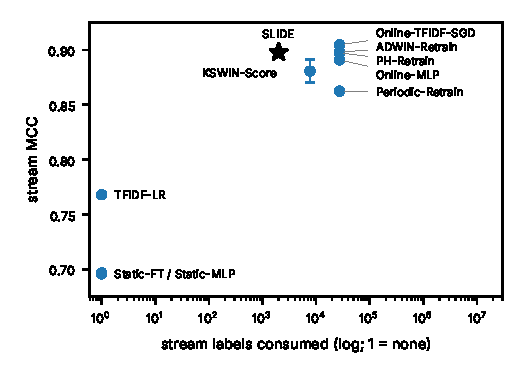
\includegraphics[width=0.62\linewidth]{figures/pareto.pdf}
\caption{Stream MCC against stream labels consumed (mean and 95\% CI over 10 realisations; static methods plotted at one label). Only the label-on-alarm methods lie between the static and the fully supervised clusters; KSWIN-Score buys 3.85 times more labels than SLIDE for a lower MCC. Static-FT and Static-MLP overlap at the bottom left.}
\label{fig:pareto}
\end{figure}

Figure~\ref{fig:pareto} places these results on the label-cost axis. KSWIN-Score uses the same purchase size as SLIDE but buys 7{,}700 labels and ends lower (0.881); Periodic retraining with all labels stays below both (0.862). Table~\ref{tab:stats} gives the paired tests. The Friedman test rejects equal performance across the ten methods ($\chi^2_F=81.91$, $p=6.8\times10^{-14}$); with a Nemenyi critical difference of 4.28 ranks, SLIDE (mean rank 3.3) is separated from TFIDF-LR (8.0) and the two static transformer detectors (9.7 and 9.3) but from no adaptive method. The realisation-level Wilcoxon tests are sharper. SLIDE wins all ten paired realisations against the three static detectors and against Periodic retraining, each at the smallest Holm-adjusted $p$-value the design allows (0.0176), and it loses all ten against Online-TFIDF-SGD at the same $p$-value. Against ADWIN-Retrain and PH-Retrain it wins five and six realisations ($p_{\mathrm{Holm}}=1$). Two comparisons sit near the threshold. SLIDE exceeds Online-MLP by 0.007 MCC in eight of ten realisations ($p_{\mathrm{Holm}}=0.039$) and KSWIN-Score by 0.017 in eight of ten, a difference that does not reach significance ($p_{\mathrm{Holm}}=0.059$) because KSWIN-Score varies four times more across realisations.

\begin{table}[t]
\centering
\caption{SLIDE versus each competitor. $\Delta$MCC: mean paired difference; wins out of 10 realisations; two-sided Wilcoxon signed-rank tests with Holm correction on realisation-level MCC and PR-AUC ($n=10$, primary) and on batch-level MCC ($n=1120$, descriptive); $r_{rb}$: rank-biserial effect size. Friedman $\chi^2_F=81.91$, $p=6.8\times10^{-14}$; Nemenyi CD$_{0.05}=4.28$.}
\label{tab:stats}
\scriptsize
\setlength{\tabcolsep}{2.5pt}
\begin{tabular}{@{}lrrrrrrrr@{}}
\toprule
Competitor & $\Delta$MCC & wins & $p_{\mathrm{Holm}}$ & $r_{rb}$ & $p^{\mathrm{PR}}_{\mathrm{Holm}}$ & $p^{\mathrm{batch}}_{\mathrm{Holm}}$ & $r^{\mathrm{batch}}_{rb}$ & rank \\
\midrule
TFIDF-LR & +0.130 & 10 & 0.0176 & +1.00 & 0.0176 & 9.8e-102 & +0.74 & 8.0 \\
Online-TFIDF-SGD & -0.007 & 0 & 0.0176 & -1.00 & 0.0176 & 1.2e-05 & -0.17 & 1.1 \\
Static-FT & +0.202 & 10 & 0.0176 & +1.00 & 0.0176 & 3.4e-162 & +0.95 & 9.7 \\
Static-MLP & +0.201 & 10 & 0.0176 & +1.00 & 0.0176 & 5.4e-151 & +0.97 & 9.3 \\
Online-MLP & +0.007 & 8 & 0.0391 & +0.89 & 1 & 0.014 & -0.11 & 5.1 \\
Periodic-Retrain & +0.035 & 10 & 0.0176 & +1.00 & 0.0176 & 0.45 & +0.05 & 6.8 \\
ADWIN-Retrain & -0.000 & 5 & 1 & -0.02 & 1 & 0.84 & +0.03 & 3.0 \\
PH-Retrain & +0.001 & 6 & 1 & +0.13 & 1 & 0.92 & -0.00 & 3.4 \\
KSWIN-Score & +0.017 & 8 & 0.0586 & +0.82 & 0.523 & 0.36 & +0.06 & 5.3 \\
\midrule
SLIDE (rank) & & & & & & & & 3.3 \\
\bottomrule
\end{tabular}
\end{table}


The batch-level tests are descriptive. Against the four retraining policies that react to time or to error (Periodic, ADWIN, Page--Hinkley and KSWIN-Score), the 1{,}120 paired batches show no difference ($p^{\mathrm{batch}}_{\mathrm{Holm}}\ge0.36$, $|r_{rb}|\le0.06$), so the stream-level gaps come from a few transition batches, not from a uniform offset. Against Online-MLP the two summaries disagree in sign ($r_{rb}=-0.11$ at batch level): Online-MLP wins slightly more individual batches while SLIDE has the higher pooled MCC, and we claim no advantage over Online-MLP beyond the realisation-level test.

\subsection{Alarm timing against equal-budget controls}\label{sec:controls}
Timing carries most of the label value. Table~\ref{tab:controls} holds the update rule fixed and varies only when the labels are bought. Spending the same 2{,}000 labels at random batches lowers MCC to 0.786 and segment-D MCC to 0.446 ($p_{\mathrm{Holm}}=0.0078$, the smallest value attainable over four rows), whereas buying them at the first moment that 500 messages of each new segment exist, which requires knowledge of the boundaries, gives 0.902, only 0.004 above SLIDE ($p_{\mathrm{Holm}}=0.059$). The score-based trigger behaves differently. With the SLIDE update, KSWIN on the score reaches 0.891 (7{,}550 labels): it is the best method on the paraphrase segment (0.932) and among the weakest adaptive ones on segment~D (0.766), and its spread across realisations ($\pm0.017$) is almost six times that of SLIDE. Part of the gap between SLIDE and KSWIN-Score in Table~\ref{tab:main} thus comes from the update rule; the remainder, at 3.8 times the label cost, is not significant ($p_{\mathrm{Holm}}=0.557$).

\begin{table}[t]
\centering
\caption{Controls that separate the timing of label purchases from the update rule (10 realisations). All rows except KSWIN-Score use the SLIDE update; Budget-Random buys four 500-label windows at random batches, Budget-Oracle buys them as soon as 500 messages of each new segment have arrived. $p_{\mathrm{Holm}}$: two-sided Wilcoxon test against SLIDE on realisation-level MCC, Holm-corrected over the four rows.}
\label{tab:controls}
\scriptsize
\setlength{\tabcolsep}{2.5pt}
\begin{tabular}{@{}lcccccr@{}}
\toprule
Method & MCC & MCC (D) & MCC (E) & Labels & $\Delta$ & $p_{\mathrm{Holm}}$ \\
\midrule
SLIDE & 0.898\,$\pm$\,0.003 & 0.825 & 0.894 & 2000 & -- & -- \\
KSWIN-Score & 0.881\,$\pm$\,0.012 & 0.765 & 0.832 & 7700 & -0.017 & 0.0586 \\
KSWIN-Score+SLIDE-update & 0.891\,$\pm$\,0.017 & 0.766 & 0.932 & 7550 & -0.007 & 0.557 \\
Budget-Random & 0.786\,$\pm$\,0.028 & 0.446 & 0.773 & 2000 & -0.112 & 0.00781 \\
Budget-Oracle & 0.902\,$\pm$\,0.003 & 0.822 & 0.899 & 2000 & +0.004 & 0.0586 \\
\bottomrule
\end{tabular}
\end{table}


\subsection{Behaviour at segment boundaries}\label{sec:boundaries}
Figure~\ref{fig:trajectory} shows where the gaps arise. All methods coincide on segment~A, and the static detectors fall to a batch MCC near 0.2 on the LLM segment~D. SLIDE raised exactly four alarms in each of the ten streams, one per boundary and none inside segment~A: at the first batch of segments B and D in every stream, and one batch after the B$\to$C and D$\to$E boundaries in eight of ten streams. The purchased labels arrive $D=2$ batches after the alarm, and the head is updated in that same batch; until then SLIDE scores with the old head, and the dip at C$\to$D in Fig.~\ref{fig:trajectory} spans those batches. ADWIN and Page--Hinkley watch the delayed error stream instead. They alarm on average 3.5 and 3.6 times per stream, retrain on the last 1{,}000 labels instead of 500 and keep receiving every later label, which explains why they match SLIDE on segment~D with 13.75 times more labels.

\begin{figure*}[t]
\centering
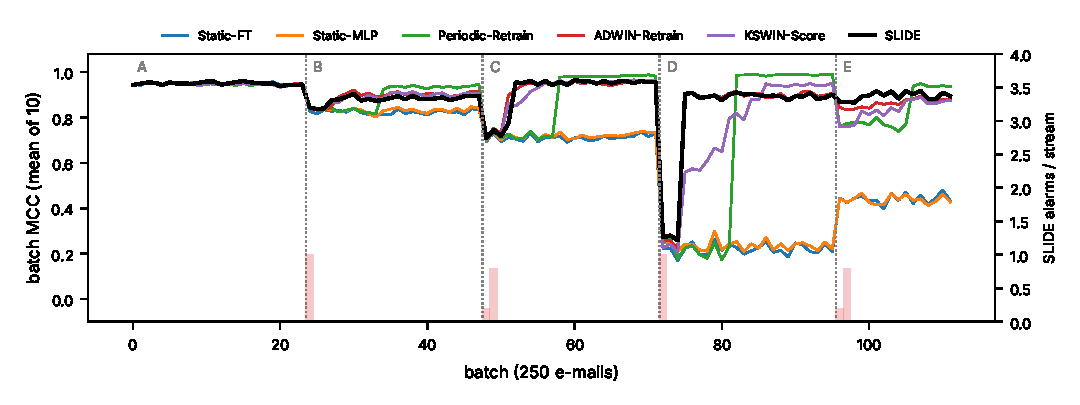
\includegraphics[width=0.95\linewidth]{figures/trajectory.pdf}
\caption{Batch MCC along the stream (mean over 10 realisations) and SLIDE alarms per batch (bars, right axis). Dotted lines mark segment boundaries.}
\label{fig:trajectory}
\end{figure*}

The two gates play distinct roles (Fig.~\ref{fig:swtrace}). At the 40 alarms the ratio $\widehat{SW}_1/\tau_\alpha$ had a median of 1.18 at A$\to$B, 1.57 at B$\to$C, 2.19 at C$\to$D and 1.33 at D$\to$E; the minimum KS $p$-value never exceeded $8.9\times10^{-5}$ and was below $10^{-7}$ at 36 of the 40 alarms. Over the 750 tests that did not alarm, the SW gate alone would never have fired, whereas the KS gate alone would have fired twelve times. KSWIN on the score stream, by comparison, triggered 15.4 refits per stream for four true changes.

\begin{figure}[t]
\centering
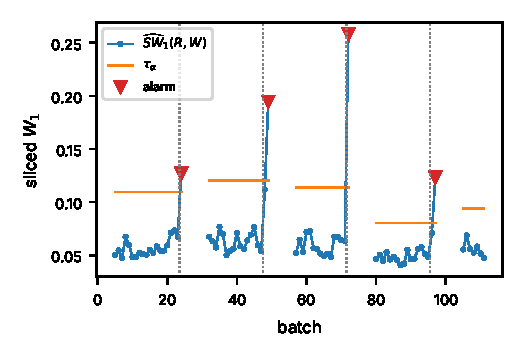
\includegraphics[width=0.62\linewidth]{figures/swtrace.pdf}
\caption{Sliced $W_1$ between reference and test window, calibrated threshold $\tau_\alpha$ and alarms for realisation 0. The threshold is re-estimated whenever the reference is rebuilt after an update; gaps mark batches without a test while the new reference and test window fill.}
\label{fig:swtrace}
\end{figure}

\begin{table}[t]
\centering
\caption{MCC per stream segment (mean over 10 realisations). Best value per column in bold.}
\label{tab:segments}
\scriptsize
\setlength{\tabcolsep}{3.5pt}
\begin{tabular}{@{}lccccc@{}}
\toprule
Method & A & B & C & D & E \\
\midrule
TFIDF-LR & \textbf{0.956} & 0.825 & 0.891 & 0.433 & 0.557 \\
Online-TFIDF-SGD & 0.925 & 0.869 & 0.920 & \textbf{0.892} & \textbf{0.897} \\
Static-FT & 0.948 & 0.824 & 0.711 & 0.221 & 0.442 \\
Static-MLP & 0.951 & 0.831 & 0.720 & 0.237 & 0.439 \\
Online-MLP & 0.946 & 0.889 & \textbf{0.924} & 0.768 & 0.895 \\
Periodic-Retrain & 0.947 & 0.892 & 0.867 & 0.711 & 0.831 \\
ADWIN-Retrain & 0.951 & 0.892 & 0.916 & 0.827 & 0.863 \\
PH-Retrain & 0.951 & \textbf{0.899} & 0.911 & 0.827 & 0.856 \\
KSWIN-Score & 0.946 & 0.888 & 0.910 & 0.765 & 0.832 \\
SLIDE & 0.950 & 0.879 & 0.915 & 0.825 & 0.894 \\
\bottomrule
\end{tabular}
\end{table}


Per-segment MCC (Table~\ref{tab:segments}) separates the two shift types. On the generator shift (D) SLIDE reaches 0.825, level with the error-triggered detectors (0.827) and behind Online-TFIDF-SGD (0.892). On the paraphrase campaign (E) it reaches 0.894, ahead of ADWIN (0.863) and Page--Hinkley (0.856) and level with Online-TFIDF-SGD (0.897) and Online-MLP (0.895). The ablation in Section~\ref{sec:ablation} does not attribute the segment-E advantage to any single term of the objective.

\subsection{Authorship slices}\label{sec:slices}
The style confound of Section~\ref{sec:audit} is visible in every transformer detector. Table~\ref{tab:slices} shows that SLIDE recovers 88.0\% of LLM-written phishing in segment~D and 93.7\% of paraphrased phishing in segment~E, whereas the static fine-tuned encoder detects 20.7\% and 36.5\%. SLIDE also flags 15.7\% of LLM-written \emph{legitimate} messages in segment~D, against 2.8\% of the human legitimate mail that sits in the same batches. Every transformer head shows the same pattern, with FPR on LLM-written legitimate mail between 6.8\% (Periodic retraining, at lower recall) and 27.0\% (Static-MLP). Online-TFIDF-SGD reaches comparable recall at 4.4\% FPR on that slice. Once it has seen every label, a word-level online model separates intent from style better than any frozen-encoder head here, and this is the largest gap in favour of a baseline that we observe.

\begin{table}[t]
\centering
\caption{Recall on malicious and FPR on legitimate messages by authorship inside segments D and E (mean over realisations; segment D contains no human-written malicious mail). ``llm'' = LLM-written, ``para'' = T1-paraphrased (malicious and the legitimate control).}
\label{tab:slices}
\scriptsize
\setlength{\tabcolsep}{2.5pt}
\begin{tabular}{@{}lccccc@{}}
\toprule
 & \multicolumn{2}{c}{Recall} & \multicolumn{3}{c}{FPR} \\
\cmidrule(lr){2-3}\cmidrule(lr){4-6}
Method & D:llm & E:para & D:llm & D:human & E:para \\
\midrule
TFIDF-LR & 0.602 & 0.670 & 0.517 & 0.080 & 0.494 \\
Online-TFIDF-SGD & 0.887 & 0.914 & 0.044 & 0.008 & 0.044 \\
Static-FT & 0.207 & 0.365 & 0.184 & 0.028 & 0.158 \\
Static-MLP & 0.272 & 0.418 & 0.270 & 0.044 & 0.252 \\
Online-MLP & 0.841 & 0.934 & 0.217 & 0.034 & 0.204 \\
Periodic-Retrain & 0.662 & 0.810 & 0.068 & 0.013 & 0.055 \\
ADWIN-Retrain & 0.875 & 0.901 & 0.135 & 0.028 & 0.168 \\
PH-Retrain & 0.876 & 0.892 & 0.137 & 0.028 & 0.165 \\
KSWIN-Score & 0.779 & 0.859 & 0.114 & 0.023 & 0.192 \\
SLIDE & 0.880 & 0.937 & 0.157 & 0.028 & 0.185 \\
\bottomrule
\end{tabular}
\end{table}


\subsection{Adversarial stress test}\label{sec:stress}
The stress pool (600 held-out phishing e-mails, Table~\ref{tab:pools}) is scored by each detector as it stands before the stream ($t_0$) and just before segment~E (pre-E), under each attack of Section~\ref{sec:threat}. The paraphraser met the attacker's constraint in most cases. The median MiniLM similarity of the rewrites was 0.912 and 96.6\% reached the 0.70 threshold within three attempts; the remaining 3.4\% keep their original text, as the threat model requires. The median word-level edit fraction was 0.58.

\begin{table*}[t]
\centering
\caption{Stress test on the held-out phishing pool: detection rate (recall at 0.5) before the stream ($t_0$) and at the D$\to$E boundary (pre-E), mean over 10 realisations.}
\label{tab:stress}
\scriptsize
\setlength{\tabcolsep}{2.5pt}
\resizebox{\textwidth}{!}{\begin{tabular}{@{}lcccccccccccccc@{}}
\toprule
 & \multicolumn{7}{c}{$t_0$ (warm-up model)} & \multicolumn{7}{c}{pre-E (after segments A--D)} \\
\cmidrule(lr){2-8}\cmidrule(lr){9-15}
Method & orig. & T1 & T2 .05 & T2 .10 & T2 .20 & T3 & T1$\circ$T2 & orig. & T1 & T2 .05 & T2 .10 & T2 .20 & T3 & T1$\circ$T2 \\
\midrule
TFIDF-LR & 0.712 & 0.645 & 0.705 & 0.687 & 0.698 & 0.448 & 0.650 & 0.712 & 0.645 & 0.705 & 0.687 & 0.698 & 0.448 & 0.650 \\
Online-TFIDF-SGD & 0.703 & 0.661 & 0.703 & 0.692 & 0.688 & 0.481 & 0.657 & 0.797 & 0.758 & 0.789 & 0.787 & 0.772 & 0.617 & 0.742 \\
Static-FT & 0.417 & 0.355 & 0.465 & 0.497 & 0.532 & 0.067 & 0.430 & 0.417 & 0.355 & 0.465 & 0.497 & 0.532 & 0.067 & 0.430 \\
Static-MLP & 0.462 & 0.407 & 0.509 & 0.527 & 0.556 & 0.103 & 0.480 & 0.462 & 0.407 & 0.509 & 0.527 & 0.556 & 0.103 & 0.480 \\
Online-MLP & 0.462 & 0.407 & 0.509 & 0.527 & 0.556 & 0.103 & 0.480 & 0.908 & 0.880 & 0.920 & 0.918 & 0.912 & 0.058 & 0.882 \\
Periodic-Retrain & 0.462 & 0.407 & 0.509 & 0.527 & 0.556 & 0.103 & 0.480 & 0.681 & 0.684 & 0.676 & 0.672 & 0.645 & 0.046 & 0.639 \\
ADWIN-Retrain & 0.462 & 0.407 & 0.509 & 0.527 & 0.556 & 0.103 & 0.480 & 0.938 & 0.897 & 0.948 & 0.937 & 0.900 & 0.099 & 0.874 \\
PH-Retrain & 0.462 & 0.407 & 0.509 & 0.527 & 0.556 & 0.103 & 0.480 & 0.938 & 0.897 & 0.948 & 0.937 & 0.900 & 0.099 & 0.874 \\
KSWIN-Score & 0.462 & 0.407 & 0.509 & 0.527 & 0.556 & 0.103 & 0.480 & 0.719 & 0.698 & 0.721 & 0.718 & 0.709 & 0.049 & 0.677 \\
SLIDE & 0.459 & 0.406 & 0.506 & 0.529 & 0.556 & 0.101 & 0.484 & 0.948 & 0.914 & 0.955 & 0.948 & 0.907 & 0.106 & 0.897 \\
\bottomrule
\end{tabular}}
\end{table*}


Table~\ref{tab:stress} supports three observations and one negative result. Paraphrase is the most effective content-preserving attack: T1 lowers SLIDE's detection rate from 0.948 to 0.914 at pre-E and from 0.459 to 0.406 at $t_0$. Character perturbation alone is weak. At $t_0$ higher rates even \emph{raise} detection for every transformer head (0.459 to 0.556 for SLIDE); homoglyphs and zero-width characters are rare in legitimate mail, so they act as a malicious signal. After adaptation SLIDE has the highest detection rate in five of the seven pre-E columns, with 0.914 under T1 and 0.897 under T1$\circ$T2 against 0.897 and 0.874 for ADWIN-Retrain; Online-MLP is ahead at $\epsilon_{\mathrm{char}}=0.20$ (0.912 against 0.907). Benign padding is the negative result. A 400-character legitimate prefix lowers the detection rate of every transformer-based method to 0.046--0.106 at both time points, whereas the TF-IDF models, which read the whole message, keep 0.45--0.62.

\begin{table}[t]
\centering
\caption{Left: displacement $\lVert\Phi(x')-\Phi(x)\rVert_2$ caused by each attack on the 600 stress e-mails (median, 10th--90th percentile; rel.: median ratio to $\lVert\Phi(x)\rVert_2$). Right: fraction of the stress e-mails that the warm-up head classifies correctly \emph{and} certifies by Proposition~\ref{prop:cert} at radius $\epsilon$, for a plain head and for a head trained with the adversarial term ($\lambda_a{=}0.5$, $\epsilon{=}1$).}
\label{tab:cert}
\scriptsize
\setlength{\tabcolsep}{2.5pt}
\begin{tabular}{@{}lrr@{\hspace{8pt}}lrr@{}}
\toprule
Attack & median (q10--q90) & rel. & radius $\epsilon$ & plain & adv. \\
\midrule
T1 paraphrase & 11.1 (5.4--21.9) & 0.40 & 0.25 & 0.438 & 0.435 \\
T2, $\epsilon_{\mathrm{char}}{=}0.05$ & 5.7 (2.6--10.8) & 0.21 & 0.5 & 0.415 & 0.427 \\
T2, $\epsilon_{\mathrm{char}}{=}0.10$ & 9.1 (4.8--16.0) & 0.33 & 1 & 0.358 & 0.370 \\
T2, $\epsilon_{\mathrm{char}}{=}0.20$ & 14.6 (7.7--24.5) & 0.53 & 2 & 0.167 & 0.203 \\
T3 padding & 30.8 (17.1--47.6) & 1.03 & $L_m$ & 6.04 & 5.45 \\
T1$\circ$T2 (0.10) & 14.6 (9.4--23.9) & 0.50 & recall & 0.460 & 0.465 \\
\bottomrule
\end{tabular}
\end{table}


Table~\ref{tab:cert} explains why the certificate of Proposition~\ref{prop:cert} cannot cover these attacks. The median displacement in $\Phi$ ranges from 5.7 (T2 at 0.05) through 11.1 (T1) to 30.8 (T3) standard-deviation units, i.e.\ 21--103\% of the norm of the original representation, while the head certifies at most 43.8\% of the stress e-mails at radius 0.25 and 20.3\% at radius 2. The adversarial term lowers the Lipschitz bound $L_m$ from 6.04 to 5.45 and raises the certified fraction at radii 0.5--2 (from 0.167 to 0.203 at $\epsilon=2$) at unchanged recall. That gain is real but an order of magnitude too small for text-level attacks; the observed robustness to T1 after adaptation comes from the labelled campaign data, not from the certificate.

\subsection{Ablation}\label{sec:ablation}
Table~\ref{tab:ablation} removes one component at a time. Two components carry the result. Without adaptation the detector stays at the static level (0.698). A drift test on the score alone raises only 1.5 alarms per stream (750 labels) and ends at 0.838; the projections of $\Phi$ are what make the shift visible, and the projections-only test reproduces SLIDE exactly. Of the objective's terms only the adversarial one has a measurable effect, 0.003 MCC consistent across the ten realisations ($p_{\mathrm{Holm}}=0.0176$). Removing the proximal term or the replay buffer changes nothing measurable, and neither does dropping the surprisal features $\psi$ ($|\Delta|\le0.002$, $p_{\mathrm{Holm}}\ge0.22$). Either gate alone still yields about four alarms per stream (2{,}000 labels without the KS gate, 2{,}100 without the SW gate); on this stream the conjunction mainly suppresses the occasional extra alarm.

\begin{table}[t]
\centering
\caption{Ablation over 10 realisations. $\Delta$: change of mean MCC relative to full SLIDE; $p$: Holm-corrected two-sided Wilcoxon test against full SLIDE on realisation-level MCC.}
\label{tab:ablation}
\scriptsize
\setlength{\tabcolsep}{2.5pt}
\begin{tabular}{@{}lccccrr@{}}
\toprule
Variant & MCC & PR-AUC & MCC (E) & Labels & $\Delta$ & $p_{\mathrm{Holm}}$ \\
\midrule
SLIDE & 0.898\,$\pm$\,0.003 & 0.977 & 0.894 & 2000 & -- & -- \\
SLIDE w/o adversarial term & 0.895\,$\pm$\,0.002 & 0.975 & 0.890 & 2000 & -0.003 & 0.0176 \\
SLIDE w/o replay & 0.900\,$\pm$\,0.003 & 0.977 & 0.890 & 2000 & +0.002 & 0.527 \\
SLIDE w/o proximal term & 0.899\,$\pm$\,0.003 & 0.977 & 0.894 & 2000 & +0.001 & 0.223 \\
SLIDE w/o surprisal $\psi$ & 0.898\,$\pm$\,0.004 & 0.976 & 0.895 & 2000 & -0.000 & 1 \\
SLIDE w/o KS gate & 0.898\,$\pm$\,0.003 & 0.977 & 0.894 & 2000 & +0.000 & 1 \\
SLIDE w/o SW gate & 0.899\,$\pm$\,0.003 & 0.976 & 0.900 & 2100 & +0.001 & 0.594 \\
SLIDE score-only test & 0.838\,$\pm$\,0.010 & 0.950 & 0.843 & 750 & -0.060 & 0.0176 \\
SLIDE projections-only test & 0.898\,$\pm$\,0.003 & 0.977 & 0.894 & 2000 & +0.000 & 1 \\
SLIDE w/o adaptation & 0.698\,$\pm$\,0.002 & 0.898 & 0.443 & 0 & -0.200 & 0.0176 \\
\bottomrule
\end{tabular}
\end{table}


\subsection{Sensitivity}\label{sec:sens}
SLIDE is insensitive to its test and robustness settings within the ranges of Table~\ref{tab:sens}. Over five realisations, MCC stays between 0.895 and 0.899 for $\epsilon\in[0.25,4]$, $\alpha\in[0.001,0.05]$ and $K\in\{16,256\}$, against 0.896 at the default; only $\alpha=0.05$ (2{,}200 labels) and $K=256$ (2{,}100) buy an extra window. The purchase size is the one lever with a visible trade-off. At $n_\ell=250$ SLIDE spends 1{,}000 labels and loses 0.008 MCC overall and 0.028 on the paraphrase segment; at $n_\ell=1000$ it spends 4{,}000 labels and gains 0.004 overall and 0.024 on that segment.

\begin{table}[t]
\centering
\caption{Sensitivity of SLIDE (5 realisations; default: $\epsilon=1$, $\alpha=0.01$, $n_\ell=500$, $K=64$; first row shows the default on the same 5 realisations).}
\label{tab:sens}
\scriptsize
\begin{tabular}{@{}lcccr@{}}
\toprule
Setting & MCC & MCC (E) & FPR & Labels \\
\midrule
default & 0.896 & 0.890 & 0.042 & 2000 \\
$\epsilon$=0.25 & 0.895 & 0.891 & 0.043 & 2000 \\
$\epsilon$=0.5 & 0.895 & 0.892 & 0.043 & 2000 \\
$\epsilon$=2.0 & 0.899 & 0.892 & 0.040 & 2000 \\
$\epsilon$=4.0 & 0.895 & 0.876 & 0.041 & 2000 \\
$\alpha$=0.001 & 0.895 & 0.888 & 0.042 & 2000 \\
$\alpha$=0.05 & 0.899 & 0.898 & 0.042 & 2200 \\
$n_\ell$=250 & 0.888 & 0.862 & 0.045 & 1000 \\
$n_\ell$=1000 & 0.900 & 0.914 & 0.039 & 4000 \\
$K$=16 & 0.897 & 0.893 & 0.042 & 2000 \\
$K$=256 & 0.897 & 0.893 & 0.042 & 2100 \\
\bottomrule
\end{tabular}
\end{table}


\subsection{Computational cost}\label{sec:cost}
The drift machinery is cheap; the transformers are not. Table~\ref{tab:latency} shows that one drift test costs 77\,ms per 250-message batch in isolation (0.31\,ms per e-mail) and 174\,ms inside the stream, where the reference and window buffers are also maintained; the encoder pass costs 27\,ms per e-mail on four threads and the surprisal model 72\,ms. A SLIDE update with PGD and replay takes 2.3\,s in isolation and 3.8\,s on average inside the stream, four times per stream. The persistent state at full reservoir capacity occupies 6.8\,MB. Since the ablation shows no benefit from $\psi$, dropping the surprisal model would cut the per-message cost by roughly 70\% on this stream.

\begin{table}[t]
\centering
\caption{Measured cost of each SLIDE component on one Intel Xeon Processor @ 2.10GHz (4 cores, no GPU). Transformer timings use batches of 32 e-mails of at most 128 tokens.}
\label{tab:latency}
\scriptsize
\setlength{\tabcolsep}{3pt}
\begin{tabular}{@{}>{\raggedright\arraybackslash}p{7cm}>{\raggedright\arraybackslash}p{6cm}@{}}
\toprule
Component & Cost \\
\midrule
DistilRoBERTa pass $\phi$ (1 / 4 threads) & 101.4 / 27.1 ms per e-mail \\
distilgpt2 surprisal $\psi$ (1 / 4 threads) & 240.5 / 71.6 ms per e-mail \\
Head $h_\theta$ scoring & 5.8 $\mu$s per e-mail \\
Drift test, isolated ($n_R{=}1000$, $n_W{=}500$, $K{=}64$) & 77.3 ms per batch (0.31 ms per e-mail) \\
Drift test, inside the stream & 173.8 ms per batch \\
Reference rebuild and calibration ($B{=}100$) & 0.91 s per alarm \\
Head update, plain CE / $\mathcal{L}_{\mathrm{total}}$ & 0.28 / 2.26 s per update \\
Head update inside the stream (mean) & 3.77 s per update \\
TF-IDF + LR scoring (reference) & 0.49 ms per e-mail \\
Parameters: encoder / LM / head & 82.1M / 81.9M / 198k \\
State at capacity: reservoir (2 classes $\times$ 1{,}000 $\times$ 772 float32) / reference / projections & 5.89 / 0.50 / 0.38 MB \\
\bottomrule
\end{tabular}
\end{table}

